\documentclass{IEEEtran}
\usepackage[utf8]{vietnam}

\usepackage{cite}
\usepackage{amsmath,amssymb,amsfonts}
\usepackage{graphicx}
\usepackage{textcomp,nicefrac}
\usepackage[hyphens]{url}
% Cho phép đường dẫn dài xuống dòng ở dấu "-" và giãn nhẹ, tránh tràn lề ở mục tài liệu tham khảo.
\Urlmuskip=0mu plus 1mu
\usepackage{xcolor}

% ----------------------------------------------------------------------
% BẢN v7 (21/11/2026): bản 6 trang, sửa theo nhận xét lần 4 (giả thuyết, Bonferroni, giao diện xếp hạng).
% Bản đầy đủ (khoảng 10 trang) lưu ở main_v3.ban-dai-10-trang.tex.bak.
% Hình nằm trong thư mục hinh/ (cùng cấp với tệp này).
% ----------------------------------------------------------------------

\markboth{STUDENT SCIENTIFIC RESEARCH COMMUNICATION, Volume II, 2026}
{Lu Dinh Thien \MakeLowercase{\textit{et al.}}: Predicting Ticket Sell-out Levels of Live Events on Ticketbox}

\begin{document}

\title{Predicting Ticket Sell-out Levels of Live Events on Ticketbox Using LightGBM}

\author{Lu Dinh Thien$^{1}$, Pham Thi Hanh$^{1}$, Tran The Trung$^{1*}$\\
\textit{$^{1}$Faculty of Information Technology, Industrial University of Ho Chi Minh City}\\
\textit{$^{*}$tranthetrung@iuh.edu.vn}}

\maketitle
\renewcommand{\abstractname}{Abstract}

% ======================================================================
\begin{abstract}
Event organizers commit most costs before ticket sales begin, while detailed sales data are rarely public. We build a dataset of 1,851 shows (649 of them labeled) from Ticketbox, a Vietnamese ticketing website, and label each show by the price-weighted share of its ticket tiers that are sold out after the show date. LightGBM quantile regression predicts the 10th, 50th and 90th percentiles of this share from information available when sales open, and the percentiles are converted into the probability of reaching a sales threshold, which approximates the break-even probability under an explicit assumption. On 137 test shows, the median forecast lowers the mean absolute error from 0.276 to 0.233 compared with a genre baseline and is better in all five rolling-origin splits, although the 95\% bootstrap interval still includes zero. The 10th--90th percentile interval stays close to [0, 1] because 75\% of the labels are exactly 0 or 1. The model is served through a forecasting service integrated into the organizer dashboard of NexaTicket, a ticketing platform built by the authors; because the probabilities are not yet calibrated, the dashboard reports a ranking against past shows.

\textit{Keywords} - {\normalfont Sell-out Prediction, Quantile Regression, LightGBM, Probabilistic Forecasting, Event Ticketing.}

\vspace{6pt}
\begin{center}
\textbf{DỰ BÁO MỨC ĐỘ BÁN HẾT VÉ CỦA SUẤT DIỄN TRÊN TICKETBOX BẰNG LIGHTGBM}
\end{center}

\textbf{\textit{Tóm tắt}} --- Ban tổ chức sự kiện phải cam kết phần lớn chi phí trước khi mở bán vé, trong khi dữ liệu bán vé hầu như không được công bố. Nghiên cứu xây dựng bộ dữ liệu 1.851 suất diễn (trong đó 649 suất có nhãn) từ Ticketbox, một trang bán vé tại Việt Nam; nhãn của mỗi suất là tỷ lệ giá trị các hạng vé đã hết, ghi nhận sau ngày diễn. Mô hình hồi quy phân vị LightGBM dự báo các phân vị 10\%, 50\% và 90\% của tỷ lệ này từ thông tin có sẵn khi mở bán; ba phân vị được chuyển thành xác suất đạt một ngưỡng bán, xấp xỉ xác suất hòa vốn dưới một giả định được nêu rõ. Trên 137 suất kiểm tra, dự báo trung vị giảm sai số tuyệt đối trung bình (MAE) từ 0,276 xuống 0,233 so với mô hình cơ sở theo thể loại và tốt hơn ở cả năm lần chia theo thời gian, dù khoảng tin cậy bootstrap 95\% vẫn chứa 0. Khoảng dự báo 10\%--90\% vẫn gần phủ trọn đoạn [0, 1] do 75\% nhãn bằng đúng 0 hoặc 1. Mô hình được tích hợp vào trang quản trị dành cho ban tổ chức của NexaTicket, nền tảng bán vé do nhóm nghiên cứu xây dựng; vì xác suất chưa được hiệu chỉnh, giao diện hiển thị thứ hạng so với các suất đã diễn.

\textit{Từ khóa} - {\normalfont Dự báo mức độ bán hết vé, Hồi quy phân vị, LightGBM, Dự báo xác suất, Phân phối vé sự kiện.}
\end{abstract}

% ======================================================================
\section{Giới thiệu}
\label{sec:intro}
% ======================================================================
Vé các sự kiện trực tiếp như hòa nhạc, sân khấu và thể thao chủ yếu được bán qua các nền tảng trực tuyến; nền tảng và ban tổ chức nắm dữ liệu bán vé chi tiết nhưng không công bố ra ngoài. Phần lớn chi phí như thuê địa điểm, sản xuất và cát-xê là chi phí cố định, phải cam kết trước khi mở bán, trong khi việc ra quyết định vẫn dựa nhiều vào kinh nghiệm. Ban tổ chức vì vậy không biết sớm sự kiện có bán đủ vé để hòa vốn hay không. Các nghiên cứu về dự báo vé sự kiện~\cite{putler2003,suher2008,fang2017,fotache2021} chủ yếu đưa ra dự báo điểm, không cho biết mức độ chắc chắn, và trong phạm vi tài liệu nhóm nghiên cứu khảo sát, chưa thấy nghiên cứu nào cho thị trường Việt Nam.

Nghiên cứu gắn với NexaTicket, nền tảng phân phối vé theo kiến trúc vi dịch vụ do nhóm nghiên cứu xây dựng. NexaTicket chưa vận hành thương mại nên chưa có dữ liệu bán thật; trước nghiên cứu này, trang thống kê dành cho ban tổ chức chỉ hiển thị số vé đã bán. Vì vậy, nhóm nghiên cứu xây dựng bộ dữ liệu từ trang bán vé công khai Ticketbox: trang này không cho biết số vé đã bán nhưng cho biết từng hạng vé còn hay đã hết. Tỷ lệ giá trị các hạng vé đã hết được dùng làm đại lượng đo mức độ bán hết vé; hồi quy phân vị với LightGBM~\cite{koenker1978,ke2017} dự báo khoảng giá trị của đại lượng này, rồi chuyển thành xác suất đạt một ngưỡng bán. Bài báo kiểm tra ba giả thuyết:
\begin{itemize}
\item \textbf{H1:} Dự báo trung vị của LightGBM có MAE thấp hơn mô hình cơ sở theo thể loại.
\item \textbf{H2:} Khoảng từ phân vị 10\% đến 90\% đủ hẹp để phân biệt các suất diễn; nhóm nghiên cứu lấy tiêu chí độ rộng trung bình dưới 0,5, tức nửa thang đo.
\item \textbf{H3:} Xác suất đạt ngưỡng suy ra từ ba phân vị phân biệt suất đạt và không đạt ngưỡng tốt hơn mô hình cơ sở.
\end{itemize}

Đóng góp chính gồm: (1) bộ dữ liệu Ticketbox với quy trình thu thập và chuẩn hóa chạy lại được, kèm phân tích phân phối nhãn và đối chiếu thủ công 20 suất; (2) quy trình dự báo phân vị bằng LightGBM có chống rò rỉ dữ liệu, chia tập theo thời gian, được đánh giá bằng bootstrap, nhiều mốc thời gian, learning curve và ablation; (3) cách chuyển ba phân vị thành xác suất đạt ngưỡng, đánh giá bằng Brier score và AUC; (4) hệ thống thu thập tự động, huấn luyện và dịch vụ dự báo tích hợp vào NexaTicket, kèm 121 kiểm thử tự động.

% ======================================================================
\section{Công trình liên quan}
\label{sec:related}
% ======================================================================
Hướng tiếp cận sớm nhất dùng số vé bán trong những ngày đầu để suy ra tổng số vé. Putler và Lele~\cite{putler2003} đề xuất khung dự báo dễ triển khai cho nghệ thuật biểu diễn; Suher~\cite{suher2008} mô hình hóa thời điểm mua vé bằng phân phối Weibull trên 13 sự kiện; Fang~\cite{fang2017} so sánh Weibull với mạng nơ-ron tự hồi quy trên bốn kỳ triển lãm hàng không. Fotache và cộng sự~\cite{fotache2021} dùng rừng ngẫu nhiên và XGBoost với các biến như thời tiết, lịch thi đấu, đội khách và phong độ đội nhà để dự báo doanh số vé 83 trận sân nhà của một câu lạc bộ bóng đá Romania, đạt $R^2$ khoảng 0,82 trên tập kiểm tra. Các công trình này kiểm tra trên số ít sự kiện, dựa vào dữ liệu bán vé nội bộ và chỉ đưa ra dự báo điểm. Trong quản trị doanh thu khách sạn, Weatherford và Kimes~\cite{weatherford2003} cho thấy các phương pháp pickup đơn giản cạnh tranh tốt với phương pháp phức tạp, nên một mô hình học máy cần được so sánh với mô hình cơ sở đơn giản.

Hồi quy phân vị~\cite{koenker1978} ước lượng trực tiếp các phân vị có điều kiện của biến mục tiêu. LightGBM~\cite{ke2017} là thư viện gradient boosting trên cây quyết định, hỗ trợ sẵn hàm mục tiêu phân vị~\cite{lgbmdoc} và được dùng rộng rãi trong các lời giải tốt nhất của cuộc thi M5~\cite{makridakis2022}. Dự báo xác suất được đánh giá bằng pinball loss kết hợp độ phủ của khoảng~\cite{gneiting2007}, và có thể hiệu chỉnh bằng phương pháp conformal~\cite{romano2019}. Trong phạm vi tài liệu nhóm nghiên cứu khảo sát, chưa thấy nghiên cứu nào chuyển dự báo vé sự kiện thành xác suất đạt một ngưỡng bán, và chưa thấy nghiên cứu nào cho thị trường Việt Nam.

% ======================================================================
\section{Thu thập và chuẩn hóa dữ liệu}
\label{sec:data}
% ======================================================================
\subsection{Thu thập}
Ba công cụ Python lần lượt lấy thông tin sự kiện, suất diễn và hạng vé từ Ticketbox~\cite{ticketbox}; chụp trạng thái từng hạng vé (còn vé, sắp hết, hết vé, ngừng bán, chưa mở bán, không rõ), mỗi hạng tối đa một lần mỗi ngày, không ghi đè dữ liệu cũ; và lưu dữ liệu thành tệp CSV và xuất ra Excel để kiểm tra. Ngoài các lần chụp, lần thu thập mở rộng ngày 18/11/2026 lấy thêm các sự kiện Ticketbox liệt kê là đã diễn ra, cùng trạng thái hạng vé tại thời điểm đó; phần lớn suất có nhãn đến từ lần này, 41 sự kiện không truy cập được vì trang đã bị gỡ. Lần chụp đầu chạy thủ công ngày 03/11/2026, lịch tự động hằng ngày chỉ có từ 18/11/2026, nên dữ liệu 04/11--17/11 bị thiếu. Do đó nhãn là ảnh chụp tại một thời điểm sau ngày diễn, chưa phải chuỗi theo thời gian.

\textit{Tuân thủ và đạo đức dữ liệu.} Công cụ đọc robots.txt ở mỗi lần thu thập, tuân theo các đường dẫn bị chặn và dừng nếu không đọc được; khi kiểm tra lại ngày 21/11/2026, tệp này chỉ chặn các đường dẫn tài khoản, đăng nhập, đăng ký và thanh toán. Công cụ không đăng nhập, nghỉ ngẫu nhiên 2--4 giây giữa hai lần truy cập và không lấy dữ liệu cá nhân. Điều khoản sử dụng của Ticketbox~\cite{ticketboxtos} không quy định riêng về thu thập tự động nhưng cấm dùng nội dung trang cho mục đích thương mại khi chưa được cho phép (mục 3.1); vì vậy dữ liệu chỉ dùng cho nghiên cứu phi thương mại, dữ liệu thô không được công bố lại, và mô hình trong NexaTicket chỉ phục vụ thử nghiệm. Mã nguồn (không kèm dữ liệu) được công khai tại \url{https://github.com/uchihathien/Concert-Ticket-Platform}, thư mục \texttt{research/forecast-data}.

\subsection{Chuẩn hóa và thống kê}
Các suất ghi trùng (cùng sự kiện, ngày và giờ diễn) được gộp (30 nhóm). Một suất thuộc phạm vi nghiên cứu khi thể loại là Nhạc sống, Sân khấu \& Nghệ thuật hoặc Thể thao (cùng là sự kiện trực tiếp bán vé có giới hạn chỗ) và địa điểm không phải trực tuyến. Đến 18/11/2026, bộ dữ liệu gồm 910 sự kiện, 1.851 suất diễn và 7.564 hạng vé. Qua các bước lọc, còn 840 suất thuộc phạm vi, 760 suất đã diễn trước lần chụp cuối, 656 suất có ít nhất một lần chụp sau ngày diễn, và 649 suất có nhãn sau khi loại 7 suất miễn phí. Ngày diễn của 649 suất kéo dài từ 10/2025 đến 11/2026; có 456 suất tại TP. Hồ Chí Minh, 112 tại Hà Nội, 81 ở nơi khác; 367 suất Nhạc sống, 235 Sân khấu \& Nghệ thuật và 47 Thể thao. Sức chứa của 339 địa điểm chưa được tra cứu.

Phân phối nhãn rất lệch về hai đầu (Hình~\ref{fig:label}): 334 suất (51,5\% số suất) có $y_i = 0$, 153 suất (23,6\%) có $y_i = 1$ và chỉ 162 suất (25,0\%) nằm giữa, tức 75\% nhãn bằng đúng 0 hoặc 1.

\begin{figure}[!t]
\centering
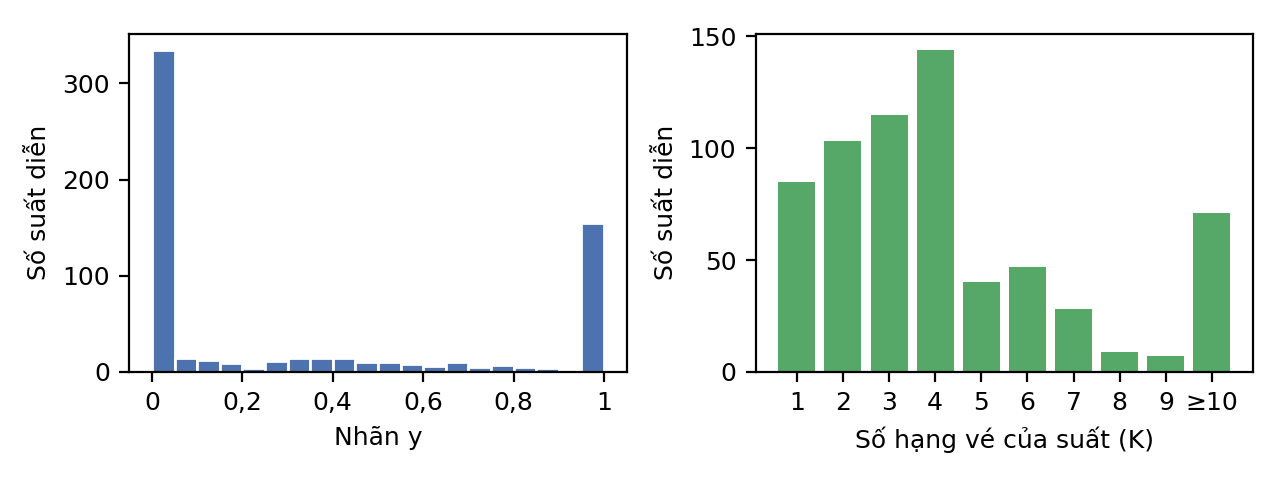
\includegraphics[width=\columnwidth]{hinh/phan_bo_nhan.png}
\caption{Phân phối nhãn $y$ (trái) và số hạng vé mỗi suất (phải) trên 649 suất có nhãn.}
\label{fig:label}
\end{figure}

% ======================================================================
\section{Phương pháp}
\label{sec:method}
% ======================================================================
\subsection{Nhãn dự báo}
Xét suất diễn $i$ có các hạng vé $k = 1, \ldots, K_i$ với giá $p_{ik}$; $h_{ik} = 1$ nếu hạng $k$ ở trạng thái hết vé và $h_{ik} = 0$ với mọi trạng thái khác. Nhãn là tỷ lệ giá trị các hạng vé đã hết:
\begin{equation}
y_i = \frac{\sum_{k=1}^{K_i} p_{ik}\, h_{ik}}{\sum_{k=1}^{K_i} p_{ik}}, \qquad 0 \leq y_i \leq 1,
\label{eq:label}
\end{equation}
với $h_{ik}$ lấy ở lần chụp đầu tiên sau ngày diễn. Trọng số chỉ là giá vì trang không công bố số lượng vé từng hạng. Sau ngày diễn, gần như mọi hạng vé chỉ ở trạng thái hết vé hoặc ngừng bán, nên $y_i$ thực chất phân biệt hạng đã bán hết với hạng bị đóng bán khi còn vé. Cần lưu ý $y_i$ không đo số vé đã bán: một suất bán 80\% vé ở mọi hạng nhưng không hạng nào hết vẫn có $y_i = 0$.

\subsection{Đặc trưng, chống rò rỉ và chia tập}
Vectơ đặc trưng gồm 10 thông tin có sẵn khi mở bán: thể loại, nhóm thành phố, số suất của sự kiện; số hạng vé, giá thấp nhất, giá cao nhất và tỷ lệ giữa hai giá; thứ trong tuần, giờ diễn và số ngày từ mở bán đến ngày diễn. Sức chứa và tín hiệu bán 7 ngày đầu đã được hỗ trợ trong mã nguồn nhưng chưa có dữ liệu nên bị bỏ tự động (đặc trưng chỉ được dùng khi có dữ liệu ở ít nhất 30\% suất huấn luyện); Ticketbox không ghi nghệ sĩ thành trường riêng và thông tin ban tổ chức chưa được thu thập. Số hạng vé và giá được lấy từ trang sự kiện tại thời điểm thu thập, với suất đã diễn là sau ngày diễn; nhóm nghiên cứu giả định chúng không đổi kể từ khi mở bán. Trạng thái hết vé chỉ dùng để tạo nhãn; bộ mã hóa, việc chọn đặc trưng và phân vị của mô hình cơ sở chỉ tính trên tập huấn luyện; siêu tham số được cố định trước, không tinh chỉnh trên tập kiểm tra.

Dữ liệu được chia theo thời gian tại ngày 26/09/2026: 512 suất trước ngày này để huấn luyện và 137 suất để kiểm tra; các suất cùng ngày luôn nằm cùng tập và không sự kiện nào có suất ở cả hai tập. Để kết quả không phụ thuộc một ngày chia, mô hình còn được đánh giá theo nhiều mốc thời gian (rolling-origin) tại 50\%, 60\%, 70\%, 80\% và 90\% số suất, mỗi lần kiểm tra trên khối khoảng 10\% số suất kế tiếp.

\subsection{LightGBM hồi quy phân vị và mô hình cơ sở}
Với mỗi $\tau \in \{0{,}1;\ 0{,}5;\ 0{,}9\}$, một mô hình LightGBM riêng được huấn luyện với hàm mất mát pinball
\begin{equation}
L_\tau(y, \hat{q}) =
\begin{cases}
\tau\,(y - \hat{q}), & y \geq \hat{q},\\
(1-\tau)\,(\hat{q} - y), & y < \hat{q},
\end{cases}
\label{eq:pinball}
\end{equation}
mà giá trị làm cực tiểu kỳ vọng chính là phân vị $\tau$ của $y$~\cite{koenker1978}. Do dữ liệu ít, cây được giới hạn nhỏ: \texttt{num\_leaves} $= 7$, \texttt{max\_depth} $= 3$, \texttt{min\_data\_in\_leaf} $= 5$, tốc độ học 0,05, 200 vòng lặp. Ba dự báo của mỗi suất được sắp xếp lại tăng dần và cắt về $[0, 1]$. Ba mô hình cơ sở dùng phân vị thực nghiệm của $y$ trên tập huấn luyện: toàn cục, theo thể loại (đối chứng chính) và theo thể loại kết hợp nhóm thành phố.

\subsection{Xác suất đạt ngưỡng và ứng dụng cho hòa vốn}
Với ngưỡng $t \in [0, 1]$, xác suất đạt ngưỡng là $P_i(t) = \Pr(y_i \geq t)$. Hàm phân phối $\hat{F}_i$ được xấp xỉ bằng nội suy tuyến tính qua $(0; 0)$, $(\hat{q}_{0{,}1}; 0{,}1)$, $(\hat{q}_{0{,}5}; 0{,}5)$, $(\hat{q}_{0{,}9}; 0{,}9)$ và $(1; 1)$; khi hai phân vị bằng nhau, xác suất giữa chúng dồn tại điểm đó. Khi đó
\begin{equation}
P_i(t) = 1 - \hat{F}_i\big(t^{-}\big),
\label{eq:pbe}
\end{equation}
nên khối xác suất đúng tại $t$ được tính là đạt ngưỡng. Cách nội suy này biểu diễn được khối xác suất tại 0 khi $\hat{q}_{0{,}1} = 0$ nhưng không biểu diễn được khối tại 1 khi $\hat{q}_{0{,}9} < 1$, nên nhóm nghiên cứu so sánh thêm với một bộ phân loại LightGBM dự báo trực tiếp biến cố $y_i \geq t$.

Gọi $C_i$ là tổng chi phí cố định và $V_i$ là doanh thu ban tổ chức nhận được nếu bán hết mọi hạng vé, đã trừ phí nền tảng và thuế. Ngưỡng hòa vốn là $y^{BE}_i = C_i / V_i$; nếu $C_i > V_i$, xác suất được quy định bằng 0. $P_i(y^{BE}_i)$ chỉ là xác suất hòa vốn dưới giả định A1: \textit{tỷ lệ giá trị các hạng vé đã hết xấp xỉ tỷ lệ doanh thu thực bán}. A1 chưa được kiểm chứng, nên trong bài $P_i$ được gọi là xác suất đạt ngưỡng bán và hòa vốn chỉ là ví dụ ứng dụng.

\subsection{Độ đo đánh giá}
Dự báo trung vị được đo bằng $\mathrm{MAE} = \frac{1}{n}\sum_{i} |y_i - \hat{q}_{0{,}5,i}|$; từng phân vị được đo bằng pinball loss trung bình theo~\eqref{eq:pinball}. Khoảng 10\%--90\% được đo bằng độ phủ (tỷ lệ suất có $y_i$ nằm trong khoảng, lý tưởng là 80\%) kèm độ rộng trung bình, vì khoảng $[0, 1]$ luôn phủ được giá trị thực nhưng vô ích cho ra quyết định~\cite{gneiting2007}. Mức chênh lệch được kiểm tra bằng bootstrap ghép cặp 5.000 lần trên tập kiểm tra. Xác suất đạt ngưỡng được đo bằng Brier score (càng nhỏ càng tốt) và AUC (0,5 là ngẫu nhiên).

% ======================================================================
\section{Hệ thống, triển khai và kiểm thử}
\label{sec:system}
% ======================================================================
\subsection{Kiến trúc và tích hợp vào NexaTicket}
Hình~\ref{fig:arch} trình bày luồng xử lý. Dữ liệu được lưu thành các tệp CSV và xuất ra Excel để kiểm tra; với quy mô hiện tại, CSV là đủ, khi chạy lâu dài nên chuyển sang cơ sở dữ liệu như PostgreSQL. Mô-đun huấn luyện lưu ba mô hình phân vị cùng bộ mã hóa. Dịch vụ dự báo viết bằng Python (máy chủ HTTP thư viện chuẩn, LightGBM, NumPy) nhận thông tin một suất qua \texttt{POST /api/du-bao}, tính đặc trưng bằng đúng hàm dùng khi huấn luyện, rồi trả về ba phân vị, ngưỡng $C/V$ và xác suất theo~\eqref{eq:pbe}; dữ liệu nhập sai bị từ chối kèm thông báo. Dịch vụ không có cơ chế đăng nhập nên chỉ nhận kết nối từ 127.0.0.1.

\begin{figure}[!t]
\centering
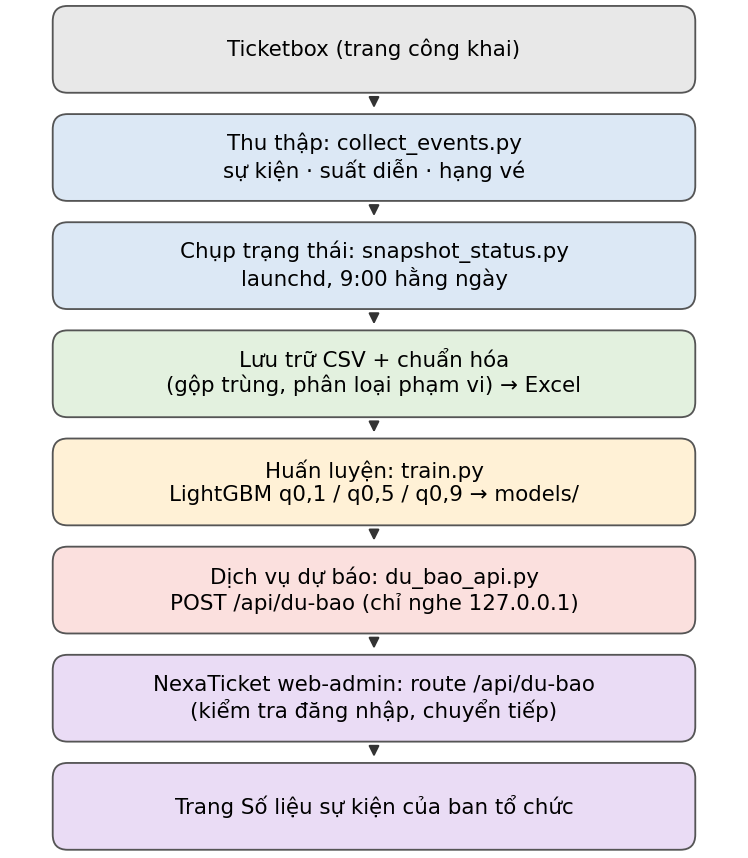
\includegraphics[width=0.8\columnwidth]{hinh/kien_truc.png}
\caption{Luồng xử lý của hệ thống, từ thu thập dữ liệu đến trang quản trị NexaTicket.}
\label{fig:arch}
\end{figure}

Trang quản trị dành cho ban tổ chức của NexaTicket (Next.js) gọi dịch vụ qua một route nội bộ có kiểm tra đăng nhập; nếu dịch vụ không chạy, chỉ khối dự báo báo lỗi. Trên trang Số liệu sự kiện (Hình~\ref{fig:ui}), khối ``Dự báo bán hết vé'' tự lấy thông tin của suất diễn được chọn, quy đổi danh mục của NexaTicket sang ba thể loại mô hình đã học, và điền sẵn $V$ bằng tổng giá nhân số chỗ; ban tổ chức chỉ cần nhập $C$. Giá trị điền sẵn là doanh thu trước phí nền tảng và thuế, khác định nghĩa $V$ ở Mục~\ref{sec:method}; giao diện nhắc ban tổ chức tự trừ các khoản này, nếu không ngưỡng $C/V$ sẽ thấp hơn, xác suất gốc bị đẩy lên và thứ hạng có thể thay đổi; đây là sai lệch đã biết. Vì xác suất từ phân vị đang cao hơn thực tế (Hình~\ref{fig:calib}) trong khi khả năng xếp thứ tự tốt hơn (AUC 0,78--0,82), kết quả chính là thứ hạng: dịch vụ tính $P_i(C/V)$ cho suất đang xét và cho 137 suất của tập kiểm tra (dự báo ngoài mẫu), rồi báo suất đang xét cao hơn bao nhiêu phần trăm số suất đó; nhóm cao, giữa và thấp ứng với một phần ba trên cùng, ở giữa và dưới cùng. Xác suất gốc vẫn được hiện kèm ghi chú chưa hiệu chỉnh, cùng ba kịch bản bi quan, thường gặp, lạc quan ứng với ba phân vị và một câu về độ chắc chắn.

\begin{figure}[!t]
\centering
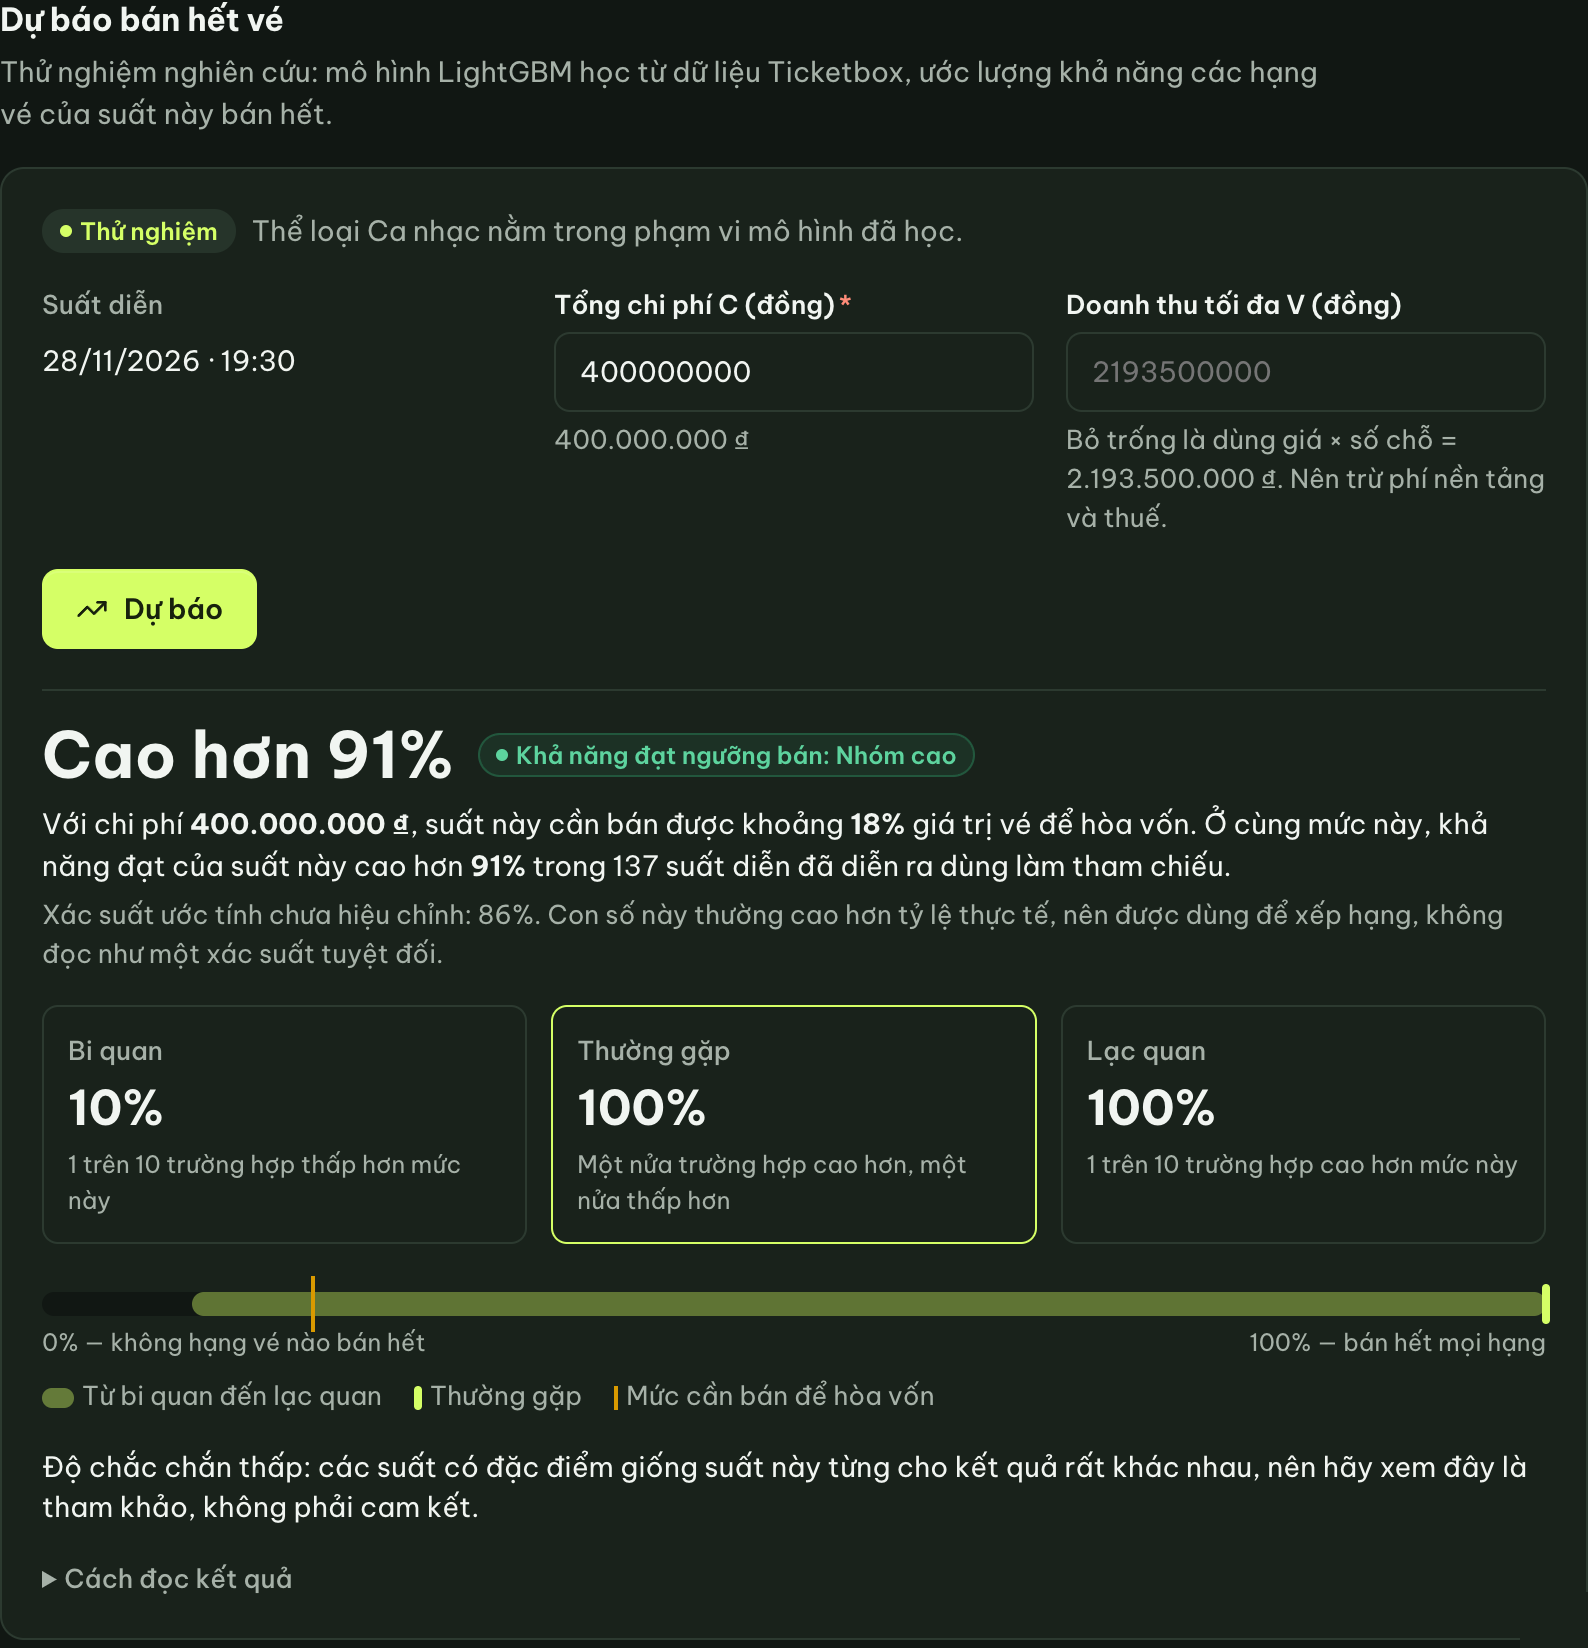
\includegraphics[width=\columnwidth]{hinh/giao_dien_xep_hang.png}
\caption{Khối Dự báo bán hết vé trên trang Số liệu sự kiện của NexaTicket.}
\label{fig:ui}
\end{figure}

\subsection{Triển khai và kiểm thử}
Hệ thống hiện chạy trong môi trường thử nghiệm cục bộ. Công cụ chụp trạng thái chạy lúc 9 giờ mỗi ngày bằng launchd trên máy cá nhân, chạy bù khi máy thức dậy và ghi nhật ký; dịch vụ dự báo khởi động cùng tập lệnh chung của NexaTicket; mô-đun huấn luyện chạy thủ công. Việc mất dữ liệu 04/11--17/11 cho thấy cần chuyển lên máy chủ (Docker và cron) kèm cảnh báo khi lỗi; hai việc này chưa được thực hiện.

\begin{table}[!t]
\caption{Một số trường hợp kiểm thử tiêu biểu (tất cả đều đạt)}
\label{tab:test}
\centering
\small
\setlength{\tabcolsep}{3pt}
\resizebox{\columnwidth}{!}{%
\begin{tabular}{|p{2.0cm}|p{3.1cm}|p{2.9cm}|}
\hline
\textbf{Chức năng} & \textbf{Đầu vào} & \textbf{Kết quả mong đợi} \\
\hline
Ánh xạ trạng thái & \texttt{sold\_out}, \texttt{sale\_closed}, \texttt{book\_now} & Hết vé, ngừng bán, còn vé \\
\hline
Tính nhãn $y$ & Hạng 300 hết vé, 100 còn vé, 600 ngừng bán & $y = 0{,}3$ \\
\hline
Chia tập & Nhiều suất cùng một ngày & Cùng nằm trong một tập \\
\hline
Xác suất đạt ngưỡng & $\hat{q} = (0{,}2; 0{,}5; 0{,}8)$; $t = 0{,}5$ và $0{,}2$ & $0{,}5$ và $0{,}9$ \\
\hline
Phân vị trùng & $\hat{q} = (0; 0; 1)$, $t = 0{,}6$ & $0{,}26$ \\
\hline
Chi phí vượt doanh thu & $C > V$ & Xác suất 0, có cảnh báo \\
\hline
Thời gian phản hồi (ngưỡng) & 50 yêu cầu liên tiếp & Phân vị 95\% dưới 200~ms \\
\hline
Route tích hợp & Gọi khi chưa đăng nhập & Chuyển về trang đăng nhập \\
\hline
\end{tabular}}
\end{table}

Hệ thống có 121 kiểm thử tự động, đều đạt: 113 kiểm thử pytest (82 cho đọc và chuẩn hóa dữ liệu, 17 cho nhãn, chia tập, đánh giá và xác suất, 14 cho dịch vụ dự báo) và 8 kiểm thử Vitest cho phần tích hợp. Bảng~\ref{tab:test} liệt kê một số trường hợp tiêu biểu; kiểm thử thời gian phản hồi trong bảng chỉ kiểm tra đạt/không đạt theo ngưỡng. Mô hình sau khi lưu và nạp lại cho dự báo trùng khớp hoàn toàn. Để đo hiệu năng thực tế, nhóm gửi riêng 200 yêu cầu thẳng đến dịch vụ trên máy cá nhân: thời gian phản hồi có trung vị 0,83~ms và phân vị 95\% là 1,07~ms.

% ======================================================================
\section{Thực nghiệm và kết quả}
\label{sec:exp}
% ======================================================================
Thực nghiệm dùng Python 3.9.6, LightGBM 4.5.0 và NumPy 2.0.2 (seed 42, chế độ deterministic), với cách chia tập và tham số ở Mục~\ref{sec:method}.

\subsection{Độ tin cậy của nhãn}
Độ trễ giữa ngày diễn và ngày gắn nhãn từ 2 đến 407 ngày (trung vị 151). Nếu Ticketbox chuyển trạng thái hàng loạt sau sự kiện, phân phối nhãn sẽ thay đổi theo độ trễ; tuy nhiên tỷ lệ $y_i = 0$ chỉ dao động 47--59\% ở bốn nhóm độ trễ ($\leq 30$, 31--90, 91--180 và $> 180$ ngày) mà không có xu hướng.

Tại thời điểm gắn nhãn, 1.710 trên 3.321 hạng vé (51,5\% số hạng vé, khác với tỷ lệ 51,5\% số suất có $y_i = 0$ ở Mục~\ref{sec:data} dù trùng giá trị) ở trạng thái hết vé, 48,3\% ngừng bán và 0,2\% còn vé; không xuất hiện các trạng thái sắp hết, chưa mở bán và không rõ. Trạng thái quyết định nhãn vì vậy là ngừng bán, được hiểu là đóng bán khi còn vé; cách hiểu này chưa được kiểm chứng bằng dữ liệu bán thật.

Một phần hiện tượng nhãn dồn hai đầu đến từ cấu trúc nhãn: suất chỉ có một hạng vé thì $y_i$ chỉ là 0 hoặc 1 (81,2\% bằng 0), nhưng ngay cả với 461 suất có từ ba hạng trở lên, vẫn có 44,3\% bằng 0 và 24,3\% bằng 1. Tương quan giữa $y_i$ và tỷ lệ số hạng vé đã hết (không trọng số) là 0,99.

Nhóm nghiên cứu chọn ngẫu nhiên phân tầng 20 suất (7 suất $y_i = 0$, 7 suất $y_i = 1$, 6 suất nằm giữa) để đối chiếu thủ công. Trạng thái đã ghi nhận khớp với trang Ticketbox ở cả 20/20 suất, cho thấy công cụ ghi nhận chính xác và trạng thái không đổi từ lần ghi nhận đến ngày đối chiếu (21/11/2026). Tuy nhiên, không tìm được nguồn độc lập nào xác nhận trực tiếp tình hình bán vé của đúng suất trong mẫu, nên tỷ lệ nhãn đúng so với thực tế chưa ước lượng được.

Trong ba suất có thông tin gián tiếp, đáng chú ý là một vở ballet tại Hà Nội: bài báo ngày 22/09/2025, hơn hai tháng trước buổi diễn, cho biết hơn 4.000 vé của năm suất diễn tại TP. Hồ Chí Minh và Hà Nội đã bán hết và ban tổ chức đã thêm một suất~\cite{vnnballet}; bài liệt kê sáu đêm (27--29/11 tại TP. Hồ Chí Minh, 03--05/12 tại Hà Nội) nhưng không nêu đêm nào là suất thêm, nên chưa xác định được suất trong mẫu (đêm cuối tại Hà Nội, 05/12/2025) thuộc năm suất đã bán hết hay là suất thêm; nhãn của suất này chỉ là 0,327 vì hạng đắt nhất (20 triệu đồng) ở trạng thái ngừng bán dù 4 trên 5 hạng đã hết. Trường hợp này cho thấy trọng số theo giá có thể làm nhãn của từng suất rất nhạy với một hạng vé đắt.

\begin{table}[!t]
\caption{Kết quả trên tập kiểm tra (137 suất diễn)}
\label{tab:result}
\centering
\small
\setlength{\tabcolsep}{3pt}
\resizebox{\columnwidth}{!}{%
\begin{tabular}{|l|c|c|c|c|}
\hline
\textbf{Độ đo} & \textbf{LightGBM} & \textbf{Thể loại} & \textbf{Toàn cục} & \textbf{TL $\times$ TP} \\
\hline
MAE của $\hat{q}_{0{,}5}$ & \textbf{0,2332} & 0,2763 & 0,2976 & 0,2719 \\
PL $\tau = 0{,}5$ & \textbf{0,1166} & 0,1382 & 0,1488 & 0,1360 \\
PL $\tau = 0{,}1$ & 0,0316 & 0,0302 & \textbf{0,0298} & 0,0302 \\
PL $\tau = 0{,}9$ & 0,0702 & 0,0702 & 0,0702 & \textbf{0,0700} \\
Độ phủ (mục tiêu 80\%) & 92,7\% & 97,8\% & 100\% & 97,8\% \\
Độ rộng trung bình & 0,97 & 1,00 & 1,00 & 0,99 \\
\hline
\multicolumn{5}{l}{\footnotesize TL $\times$ TP: theo thể loại và nhóm thành phố; PL: pinball loss.}
\end{tabular}}
\end{table}

\subsection{So sánh với các mô hình cơ sở}
Bảng~\ref{tab:result} cho thấy LightGBM có MAE thấp nhất: 0,233 so với 0,276 của mô hình cơ sở theo thể loại, tức giảm khoảng 16\%. Bootstrap cho mức giảm MAE là 0,043 với khoảng tin cậy 95\% là $[-0{,}013;\ 0{,}099]$ (6,5\% mẫu bootstrap không cho thấy LightGBM tốt hơn); với pinball loss tại $\tau = 0{,}5$ là $[-0{,}005;\ 0{,}049]$. LightGBM có xu hướng tốt hơn nhưng chưa đạt ý nghĩa thống kê ở mức 95\% với 137 suất. Ở năm lần chia theo thời gian, MAE của LightGBM lần lượt là 0,293; 0,376; 0,210; 0,248 và 0,188, so với 0,376; 0,497; 0,268; 0,291 và 0,260 của mô hình cơ sở theo thể loại, tức tốt hơn ở cả năm lần với mức chênh 0,04--0,12. H1 vì vậy chỉ được ủng hộ một phần: hướng cải thiện ổn định qua các lần chia nhưng chưa đạt ý nghĩa thống kê. Lần thứ tư dùng đúng ngày chia của Bảng~\ref{tab:result}: mốc 80\% rơi vào suất thứ 519, nhưng các suất cùng ngày 26/09/2026 được giữ chung một tập nên tập huấn luyện có 512 suất; lần này chỉ kiểm tra trên 70 suất kế tiếp nên MAE khác.

Ở phân vị 10\% và 90\%, LightGBM không tốt hơn mô hình cơ sở; tại $\tau = 0{,}9$, cả LightGBM và mô hình cơ sở theo thể loại đều dự báo $\hat{q}_{0{,}9} = 1$ cho mọi suất nên pinball loss bằng nhau. Độ phủ của mô hình cơ sở theo thể loại là 97,8\% vì phân vị 10\% của thể loại Thể thao là 0,024, khiến ba suất Thể thao có $y = 0$ nằm ngoài khoảng. Mọi phương pháp đều có độ phủ trên 80\% nhưng độ rộng 0,97--1,00, tức khoảng dự báo gần như phủ trọn $[0, 1]$; độ rộng ở năm lần chia theo thời gian cũng đều trên 0,91. Với tiêu chí độ rộng dưới 0,5, H2 bị bác bỏ.

\subsection{Xác suất đạt ngưỡng}
Bảng~\ref{tab:threshold} so sánh bốn cách ước tính xác suất đạt ngưỡng ở $t = 0{,}3;\ 0{,}5;\ 0{,}7$: từ ba phân vị của LightGBM theo~\eqref{eq:pbe}, từ ba phân vị của mô hình cơ sở theo thể loại, bộ phân loại LightGBM trực tiếp (cùng đặc trưng và tham số cây), và tỷ lệ đạt ngưỡng trong tập huấn luyện. Xác suất từ phân vị của LightGBM có AUC 0,78--0,82 và Brier score thấp hơn mô hình cơ sở ở cả ba ngưỡng. Bootstrap cho mức chênh AUC so với mô hình cơ sở là 0,118 ($[0{,}047;\ 0{,}190]$) ở $t = 0{,}3$, 0,093 ($[0{,}014;\ 0{,}174]$) ở $t = 0{,}5$ và 0,067 ($[-0{,}014;\ 0{,}151]$) ở $t = 0{,}7$, nên khi xét riêng từng ngưỡng, H3 được ủng hộ ở $t = 0{,}3$ và $0{,}5$. Ba ngưỡng là ba phép so sánh; nếu hiệu chỉnh Bonferroni (khoảng tin cậy 98,3\%), chỉ ngưỡng 0,3 còn có ý nghĩa ($[0{,}031;\ 0{,}205]$), còn ở $t = 0{,}5$ khoảng là $[-0{,}003;\ 0{,}192]$. Bộ phân loại trực tiếp có Brier score thấp hơn ở $t = 0{,}3$ và $0{,}7$ nhưng không vượt trội rõ, nên cách suy ra từ ba phân vị cho kết quả tương đương.

\begin{table}[!t]
\caption{Brier score / AUC của xác suất đạt ngưỡng trên 137 suất kiểm tra}
\label{tab:threshold}
\centering
\small
\setlength{\tabcolsep}{3pt}
\resizebox{\columnwidth}{!}{%
\begin{tabular}{|l|c|c|c|}
\hline
\textbf{Phương pháp} & \textbf{$t = 0{,}3$} & \textbf{$t = 0{,}5$} & \textbf{$t = 0{,}7$} \\
\hline
Tỷ lệ suất đạt ngưỡng & 35,8\% & 27,7\% & 22,6\% \\
\hline
LightGBM phân vị & 0,205 / \textbf{0,789} & \textbf{0,181} / \textbf{0,783} & 0,146 / 0,817 \\
LightGBM phân loại & \textbf{0,192} / 0,753 & 0,186 / 0,746 & \textbf{0,136} / \textbf{0,824} \\
Cơ sở theo thể loại & 0,224 / 0,672 & 0,194 / 0,691 & 0,168 / 0,749 \\
Tỷ lệ tập huấn luyện & 0,234 / 0,500 & 0,204 / 0,500 & 0,179 / 0,500 \\
\hline
\end{tabular}}
\end{table}

\begin{figure}[!t]
\centering
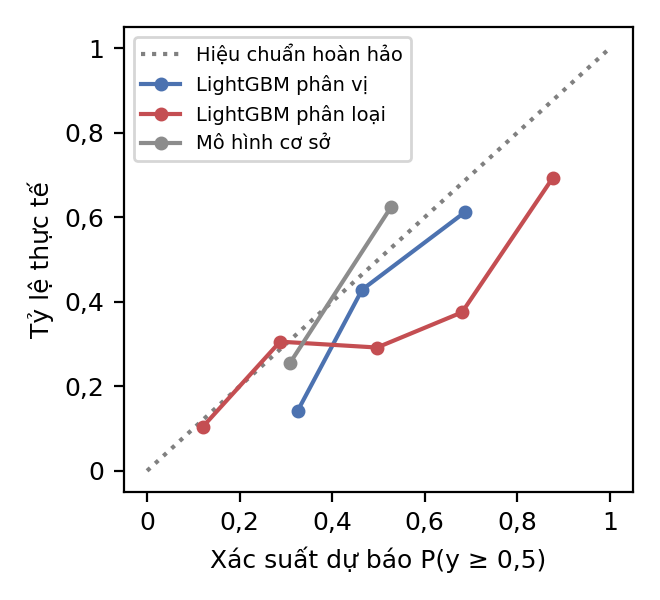
\includegraphics[width=0.8\columnwidth]{hinh/hieu_chuan.png}
\caption{Biểu đồ hiệu chuẩn của xác suất đạt ngưỡng $t = 0{,}5$ trên tập kiểm tra (chỉ vẽ các nhóm có ít nhất 3 suất).}
\label{fig:calib}
\end{figure}

Hình~\ref{fig:calib} cho thấy các điểm của xác suất từ phân vị đều nằm dưới đường chéo: tỷ lệ thực tế thấp hơn xác suất dự báo ở mọi nhóm, rõ nhất ở nhóm dự báo khoảng 0,33 (thực tế khoảng 0,14) và vẫn còn ở nhóm dự báo khoảng 0,7 (thực tế khoảng 0,6). Bộ phân loại trực tiếp còn lệch hơn ở mức xác suất cao (dự báo khoảng 0,68 và 0,88, thực tế 0,38 và 0,69), nên cách suy ra từ ba phân vị không thua kém về hiệu chuẩn. Xác suất này vì vậy phù hợp để xếp hạng các suất hơn là đọc như xác suất tuyệt đối. Ví dụ, với ngưỡng hòa vốn giả định $y^{BE} = C/V = 0{,}6$ (không phải chi phí thật), trong ba suất kiểm tra có nhãn thấp nhất, ở vị trí trung vị và cao nhất, hai suất có nhãn thật bằng 0 nhận xác suất 26\% còn suất có nhãn thật bằng 1 nhận 62\%: thứ tự đúng chiều nhưng khoảng cách chưa đủ lớn để ra quyết định.

\begin{table}[!t]
\caption{Tóm tắt kết luận về các giả thuyết}
\label{tab:hyp}
\centering
\small
\setlength{\tabcolsep}{3pt}
\resizebox{\columnwidth}{!}{%
\begin{tabular}{|l|p{4.6cm}|p{2.2cm}|}
\hline
\textbf{GT} & \textbf{Bằng chứng} & \textbf{Kết luận} \\
\hline
H1 & MAE 0,233 so với 0,276; tốt hơn ở cả 5 lần chia; khoảng tin cậy 95\% chứa 0 & Ủng hộ một phần \\
\hline
H2 & Độ rộng khoảng 0,97, vượt tiêu chí 0,5 & Bác bỏ \\
\hline
H3 & AUC cao hơn ở cả 3 ngưỡng; có ý nghĩa ở $t = 0{,}3$ và $0{,}5$ khi xét riêng, chỉ ở $t = 0{,}3$ sau hiệu chỉnh Bonferroni & Ủng hộ ở $t = 0{,}3$ \\
\hline
\end{tabular}}
\end{table}

\subsection{Learning curve, đặc trưng và ablation}
Huấn luyện lại trên phần gần nhất của tập huấn luyện với 77, 128, 256, 384 và 512 suất cho MAE lần lượt 0,280; 0,248; 0,301; 0,255; 0,233 và độ rộng khoảng 0,95; 0,88; 0,93; 0,95; 0,97: thêm dữ liệu cùng loại đặc trưng chưa làm khoảng hẹp lại. Trong mô hình trung vị, số hạng vé chiếm 46\% và tỷ lệ giá cao nhất trên giá thấp nhất chiếm 21\% tổng gain; số hạng vé quan trọng một phần vì nó gắn trực tiếp với cấu trúc nhãn. Ablation trên tập kiểm tra cho cùng kết luận: bỏ nhóm thông tin vé làm MAE tăng lên 0,264, bỏ thể loại và nhóm thành phố làm MAE tăng lên 0,265, còn bỏ nhóm thông tin thời gian làm MAE giảm nhẹ xuống 0,227. Nhóm thời gian vẫn được giữ có chủ đích, vì bỏ đặc trưng dựa trên kết quả tập kiểm tra là rò rỉ dữ liệu. Phần cải thiện so với mô hình cơ sở vì vậy chủ yếu đến từ cơ cấu hạng vé và giá, kết hợp với thể loại và thành phố. Bảng~\ref{tab:hyp} tóm tắt kết luận về ba giả thuyết.

\subsection{Phân tích và hạn chế}
Khoảng dự báo rộng có thể do hai nguyên nhân. Thứ nhất, nhãn dồn về hai đầu: khi mô hình chưa phân biệt rõ suất nào sẽ hết vé, phân vị 10\% thường bằng 0 và phân vị 90\% thường bằng 1; một phần do cấu trúc nhãn ở suất ít hạng vé, phần còn lại có thể phản ánh thị trường, nơi một hạng vé hoặc bán hết, hoặc bị đóng bán khi còn vé. Thứ hai, mô hình còn thiếu thông tin mạnh như sức chứa địa điểm và tín hiệu bán vé những ngày đầu; ảnh hưởng của chúng sẽ được kiểm tra khi có dữ liệu.

Các hạn chế chính: (1) nhãn là đại lượng xấp xỉ từ trạng thái hạng vé, không phải số vé bán thật, và giả định A1 chưa được kiểm chứng; (2) nhãn là ảnh chụp một thời điểm sau ngày diễn, chưa ước lượng được tỷ lệ nhãn đúng bằng nguồn độc lập, và trọng số theo giá có thể làm nhãn thấp hơn thực tế khi hạng đắt nhất bị ngừng bán; (3) chưa có tín hiệu bán vé giai đoạn đầu do việc chụp hằng ngày mới chạy từ 18/11/2026; (4) sức chứa, nghệ sĩ và ban tổ chức chưa được đưa vào mô hình, nên chưa kiểm tra được trường hợp cùng nghệ sĩ hoặc ban tổ chức ở cả hai tập; (5) tập kiểm tra chỉ có 137 suất; (6) một số trang sự kiện cũ đã bị gỡ; (7) dữ liệu thuộc sở hữu của Ticketbox nên chỉ dùng cho nghiên cứu phi thương mại; (8) dữ liệu chỉ từ một trang bán vé và chi phí thật không được công bố nên ví dụ hòa vốn phải dùng ngưỡng giả định.

% ======================================================================
\section{Kết luận và hướng phát triển}
\label{sec:conclusion}
% ======================================================================
Bài báo xây dựng bộ dữ liệu 910 sự kiện, 1.851 suất diễn (649 suất có nhãn) và 7.564 hạng vé từ Ticketbox, dùng tỷ lệ giá trị các hạng vé đã hết làm đại lượng đo mức độ bán hết vé, dự báo ba phân vị bằng LightGBM, chuyển thành xác suất đạt ngưỡng bán và tích hợp dịch vụ dự báo vào trang quản trị của NexaTicket. Trên 137 suất kiểm tra, dự báo trung vị giảm MAE khoảng 16\% so với mô hình cơ sở theo thể loại và tốt hơn ở cả năm lần chia theo thời gian, dù chưa đạt ý nghĩa thống kê ở mức 95\% (H1 được ủng hộ một phần); xác suất đạt ngưỡng có AUC 0,78--0,82, cao hơn mô hình cơ sở có ý nghĩa thống kê ở ngưỡng 0,3 kể cả sau hiệu chỉnh đa so sánh (H3). Khoảng dự báo vẫn gần như phủ trọn $[0, 1]$, chủ yếu do nhãn dồn về 0 và 1 (H2 bị bác bỏ). Số hạng vé chiếm 46\% tổng gain và gắn trực tiếp với cách tính nhãn, nên một phần mức cải thiện có thể phản ánh cấu trúc nhãn hơn là nhu cầu mua vé thật; vì xác suất chưa được hiệu chỉnh, giao diện hiện dùng thứ hạng thay cho xác suất tuyệt đối. Hướng phát triển gồm: xin dữ liệu bán vé từ ban tổ chức để kiểm chứng nhãn và thử nhãn không trọng số theo giá; tra cứu sức chứa địa điểm; tạo tín hiệu bán vé sớm từ dữ liệu chụp hằng ngày; đóng gói Docker và chạy việc thu thập trên máy chủ; hiệu chỉnh xác suất (isotonic hoặc Platt trên một phần tách theo thời gian từ tập huấn luyện) và hiệu chỉnh khoảng dự báo bằng phương pháp conformal~\cite{romano2019}; và khi NexaTicket có số vé bán thật, dự báo trực tiếp doanh thu, kiểm chứng giả định A1 và so sánh với phương pháp pickup.

% ======================================================================
\begin{thebibliography}{00}
\bibitem{putler2003} D. S. Putler and S. Lele, ``An easily implemented framework for forecasting ticket sales to performing arts events,'' \textit{Marketing Letters}, vol. 14, no. 4, pp. 307--320, 2003.
\bibitem{suher2008} J. Suher, ``Forecasting event ticket sales,'' Research paper, Univ. of Pennsylvania, Philadelphia, PA, USA, May 2008. [Online]. Available: \url{https://repository.upenn.edu/handle/20.500.14332/49309}
\bibitem{fang2017} Y. Fang, ``Predictive models for air show ticket sales,'' M.S. thesis, Middle Tennessee State Univ., Murfreesboro, TN, USA, 2017.
\bibitem{fotache2021} M. Fotache, I.-C. Cojocariu, and A.-F. Bertea, ``High-level machine learning framework for sports events ticket sales prediction,'' in \textit{Proc. CompSysTech '21}, ACM, 2021, pp. 55--60, doi: 10.1145/3472410.3472426.
\bibitem{koenker1978} R. Koenker and G. Bassett, ``Regression quantiles,'' \textit{Econometrica}, vol. 46, no. 1, pp. 33--50, 1978.
\bibitem{ke2017} G. Ke \textit{et al.}, ``LightGBM: A highly efficient gradient boosting decision tree,'' in \textit{Proc. NeurIPS}, 2017, pp. 3146--3154.
\bibitem{weatherford2003} L. R. Weatherford and S. E. Kimes, ``A comparison of forecasting methods for hotel revenue management,'' \textit{Int. J. Forecasting}, vol. 19, no. 3, pp. 401--415, 2003.
\bibitem{lgbmdoc} LightGBM Developers, ``Parameters --- LightGBM documentation (objective: quantile),'' [Online]. Available: \url{https://lightgbm.readthedocs.io/en/v4.5.0/Parameters.html}. Accessed: Nov. 19, 2026.
\bibitem{makridakis2022} S. Makridakis, E. Spiliotis, and V. Assimakopoulos, ``M5 accuracy competition: Results, findings, and conclusions,'' \textit{Int. J. Forecasting}, vol. 38, no. 4, pp. 1346--1364, 2022.
\bibitem{gneiting2007} T. Gneiting and A. E. Raftery, ``Strictly proper scoring rules, prediction, and estimation,'' \textit{J. Amer. Statist. Assoc.}, vol. 102, no. 477, pp. 359--378, 2007.
\bibitem{romano2019} Y. Romano, E. Patterson, and E. Candès, ``Conformalized quantile regression,'' in \textit{Proc. NeurIPS}, 2019, pp. 3543--3553.
\bibitem{ticketbox} Ticketbox, ``Ticketbox -- Nền tảng bán vé sự kiện,'' [Online]. Available: \url{https://ticketbox.vn}. Accessed: Nov. 18, 2026.
\bibitem{ticketboxtos} Công ty TNHH Ticketbox, ``Điều khoản sử dụng áp dụng cho khách hàng,'' [Online]. Available: \url{https://ticketbox.vn/customer-terms-of-use}. Accessed: Nov. 21, 2026.
\bibitem{vnnballet} VietNamNet, ``Vietnamese audience overwhelms ballet organizers with unexpected love,'' Sep. 2025. [Online]. Available: \url{https://vietnamnet.vn/en/vietnamese-audience-overwhelms-ballet-organizers-with-unexpected-love-2444802.html}. Accessed: Nov. 21, 2026.
\end{thebibliography}

\end{document}
